% ------------------------------------------------------------
% Appendix: Deriving the (negative) ELBO loss for the SeqGPLVM
% ------------------------------------------------------------

\section{SeqGPLVM loss function}
\label{sec:seqgplvm_loss}
In this section, we derive the ELBO (evidence lower bound) for the sequential Gaussian process latent variable 
model (SeqGPLVM) introduced in Section~\ref{sec:seqgplvm}. 

\subsection{Notation}
We use uppercase letters to denote random quantities and the 
corresponding lowercase letters to denote their realizations; boldface 
indicates vector or collection-valued objects, while plain letters denote 
scalars. Let \(\mathbf{X}_{it}\in\mathbb{R}^D\) denote the random covariate vector 
for individual \(i\) at time \(t\), and let \(\mathbf{x}_{it}\) denote its realization, 
where \(N\) is the number of individuals, \(D\) is the number of covariates, and \(T\) 
is the number of time points. Let \(A_{it}\in\{0,1\}\) denote the random treatment for 
individual \(i\) at time \(t\), and let \(a_{it}\) denote its realization. 
Here, we assume scalar treatments for simplicity, but the extension to multi-dimensional 
treatments is straightforward. Also, we assume a binary treatment for concreteness; 
however, this restriction is not required for the theoretical results. 
We index individuals by \(i \in \{1,\dots,N\}\) and time by \(t \in \{1,\dots,T\}\).

We let \(\mathbf{A}_t = \{A_{it}\}_{i=1}^N\) and \(\mathbf{X}_t = \{\mathbf{X}_{it}\}_{i=1}^N\) 
denote the collections of treatments and covariate vectors, respectively, 
for all individuals at time \(t\), and \(\mathbf{A}_i = \{A_{it}\}_{t=1}^T\) 
and \(\mathbf{X}_i = \{\mathbf{X}_{it}\}_{t=1}^T\) denote the corresponding 
random collections over all time points for individual \(i\). Their observed 
realizations are denoted by 
\(\mathbf{a}_t = \{a_{it}\}_{i=1}^N\), \(\mathbf{x}_t = 
\{\mathbf{x}_{it}\}_{i=1}^N\), \(\mathbf{a}_i = \{a_{it}\}_{t=1}^T\), 
and \(\mathbf{x}_i = \{\mathbf{x}_{it}\}_{t=1}^T\). Therefore, 
we write \(\mathbf{A} = \{\mathbf{A}_t\}_{t=1}^T = \{\mathbf{A}_i\}_{i=1}^N\) 
for the full random treatment collection and 
\(\mathbf{a} = \{\mathbf{a}_t\}_{t=1}^T = \{\mathbf{a}_i\}_{i=1}^N\) for its realization. 
Similarly, we write \(\mathbf{X} = \{\mathbf{X}_t\}_{t=1}^T = \{\mathbf{X}_i\}_{i=1}^N\) 
for the full random covariate collection and \(\mathbf{x} = \{\mathbf{x}_t\}_{t=1}^T = 
\{\mathbf{x}_i\}_{i=1}^N\) for its realization. We use \(\mathbf{Z} = \{\mathbf{Z}_i\}_{i=1}^N\) to denote the collection of time-invariant 
latent variables, where \(\mathbf{Z}_i \in \mathbb{R}^J\) is the 
latent variable for individual \(i\) and \(J\) is the latent dimensionality. 

We use \(\boldsymbol{\gamma}\) and \(\boldsymbol{\psi}\) to denote the 
generative and variational hyperparameters, respectively. Generative hyperparameters are 
those that define how the data is generated and enter the prior and likelihood, e.g., 
the kernel lengthscale and variance in GPs, while variational hyperparameters are those 
that define the variational family, e.g., the mean and variance in Gaussian variational 
distributions.

\subsection{Variational inference background}
\label{sec:variational_inference_background}
The ultimate inferential goal of the SeqGPLVM is to estimate the posterior distribution over 
the time-invariant latent substitute confounder \(\mathbf{Z}\) given the observed data 
\(\mathbf{x}\) and \(\mathbf{a}\). By Bayes' rule, we can write the posterior as a 
function of the likelihood and prior:
\[
p_{\boldsymbol{\gamma}}(\mathbf{z}\mid \mathbf{x},\mathbf{a})
=
\frac{
p_{\boldsymbol{\gamma}}(\mathbf{a}\mid \mathbf{x},\mathbf{z})\,
p_{\boldsymbol{\gamma}}(\mathbf{z}\mid \mathbf{x})
}{
p_{\boldsymbol{\gamma}}(\mathbf{a}\mid \mathbf{x})
}.
\]
where the denominator
\(
p_{\boldsymbol{\gamma}}(\mathbf{a}\mid \mathbf{x})
\)
(the \emph{marginal likelihood} / \emph{evidence}) is the normalizing constant. Note that 
we use \(\boldsymbol{\gamma}\) to parameterize both the likelihood and the prior to make 
the notation more concise, 
but in practice, they can have different hyperparameters.
Rewriting the logarithm of evidence as an 
integral over latent variables,  
\begin{equation}
\log p_{\boldsymbol{\gamma}}(\mathbf{a}\mid \mathbf{x}) = 
\log \int p_{\boldsymbol{\gamma}}(\mathbf{a},\mathbf{z}\mid \mathbf{x})\,\mathrm{d}\mathbf{z}.
\end{equation}
In latent-variable models this integral is typically intractable which means the 
posterior cannot be computed exactly; introducing a tractable variational density 
\(q_{\boldsymbol{\psi}}(\mathbf{z}\mid \mathbf{x})\) 
yields a lower bound on \(\log p_{\boldsymbol{\gamma}}(\mathbf{a}\mid\mathbf{x})\). 
The gap between this bound and the true log-evidence is a KL divergence to the true posterior, 
so maximizing the bound pushes \(q_{\boldsymbol{\psi}}(\mathbf{z}\mid \mathbf{x})\) 
towards \(p_{\boldsymbol{\gamma}}(\mathbf{z}\mid \mathbf{x},\mathbf{a})\). To see this, 
the marginal likelihood can be written as
\begin{align}
\log p_{\boldsymbol{\gamma}}(\mathbf{a}\mid \mathbf{x})
&= \log \int p_{\boldsymbol{\gamma}}(\mathbf{a},\mathbf{z}\mid \mathbf{x})\,\mathrm{d}\mathbf{z}
\nonumber\\
&= \log \int q_{\boldsymbol{\psi}}(\mathbf{z}\mid \mathbf{x})\,
\frac{p_{\boldsymbol{\gamma}}(\mathbf{a},\mathbf{z}\mid \mathbf{x})}{q_{\boldsymbol{\psi}}(\mathbf{z}\mid \mathbf{x})}\,
\mathrm{d}\mathbf{z}
\nonumber\\
&\ge \int q_{\boldsymbol{\psi}}(\mathbf{z}\mid \mathbf{x})
\log\frac{p_{\boldsymbol{\gamma}}(\mathbf{a},\mathbf{z}\mid \mathbf{x})}{q_{\boldsymbol{\psi}}(\mathbf{z}\mid \mathbf{x})}\,
\mathrm{d}\mathbf{z}
\;=:\; \mathcal{L}(\boldsymbol{\psi},\boldsymbol{\gamma}),
\label{eq:elbo-def}
\end{align}
where the inequality is Jensen's inequality. $\mathcal{L}(\boldsymbol{\psi},\boldsymbol{\gamma})$ 
is called the evidence lower bound (ELBO). The KL divergence 
between the variational distribution and the true posterior can be written as

\begin{align*}
    \mathrm{KL}\!\left(q_{\boldsymbol{\psi}}(\mathbf{z}\mid \mathbf{x})\,\|\,p_{\boldsymbol{\gamma}}(\mathbf{z}\mid \mathbf{x},\mathbf{a})\right)
    &= \int q_{\boldsymbol{\psi}}(\mathbf{z}\mid \mathbf{x}) \log\frac{q_{\boldsymbol{\psi}}(\mathbf{z}\mid \mathbf{x})}{p_{\boldsymbol{\gamma}}(\mathbf{z}\mid \mathbf{x},\mathbf{a})}\, \mathrm{d}\mathbf{z} \\
    &= \int q_{\boldsymbol{\psi}}(\mathbf{z}\mid \mathbf{x}) \left[ \log q_{\boldsymbol{\psi}}(\mathbf{z}\mid \mathbf{x}) - \log p_{\boldsymbol{\gamma}}(\mathbf{z}\mid \mathbf{x},\mathbf{a}) \right] \, \mathrm{d}\mathbf{z} \\
    &= \int q_{\boldsymbol{\psi}}(\mathbf{z}\mid \mathbf{x}) \left[ \log q_{\boldsymbol{\psi}}(\mathbf{z}\mid \mathbf{x}) - \log\frac{p_{\boldsymbol{\gamma}}(\mathbf{a},\mathbf{z}\mid \mathbf{x})}{p_{\boldsymbol{\gamma}}(\mathbf{a}\mid \mathbf{x})} \right] \, \mathrm{d}\mathbf{z} \\
    &= \log p_{\boldsymbol{\gamma}}(\mathbf{a}\mid \mathbf{x}) - \int q_{\boldsymbol{\psi}}(\mathbf{z}\mid \mathbf{x}) \log\frac{p_{\boldsymbol{\gamma}}(\mathbf{a},\mathbf{z}\mid \mathbf{x})}{q_{\boldsymbol{\psi}}(\mathbf{z}\mid \mathbf{x})}\, \mathrm{d}\mathbf{z} \\
    &= \log p_{\boldsymbol{\gamma}}(\mathbf{a}\mid \mathbf{x}) - \mathcal{L}(\boldsymbol{\psi},\boldsymbol{\gamma}).
\end{align*}
Equivalently,
\begin{equation}
\log p_{\boldsymbol{\gamma}}(\mathbf{a}\mid \mathbf{x})
=
\mathcal{L}(\boldsymbol{\psi},\boldsymbol{\gamma})
+
\mathrm{KL}\!\left(q_{\boldsymbol{\psi}}(\mathbf{z}\mid \mathbf{x})\,\|\,p_{\boldsymbol{\gamma}}(\mathbf{z}\mid \mathbf{x},\mathbf{a})\right).
\label{eq:logp-decomp}
\end{equation}
Maximizing \(\mathcal{L}(\boldsymbol{\psi},\boldsymbol{\gamma})\) w.r.t.\ \(q\) minimizes the 
KL divergence to the true posterior and equality 
holds iff \(q_{\boldsymbol{\psi}}(\mathbf{z}\mid \mathbf{x}) = 
p_{\boldsymbol{\gamma}}(\mathbf{z}\mid \mathbf{x},\mathbf{a})\). 
This is true since the lhs of \eqref{eq:logp-decomp} does not depend on \(q\). 
Thus, we can use \(\mathcal{L}(\boldsymbol{\psi},\boldsymbol{\gamma})\) as a surrogate objective for approximate inference. 
\(\mathcal{L}(\boldsymbol{\psi},\boldsymbol{\gamma})\) can be rewritten as 
\begin{align}
\mathcal{L}(\boldsymbol{\psi},\boldsymbol{\gamma})
&= \int q_{\boldsymbol{\psi}}(\mathbf{z}\mid \mathbf{x})\,\log\!\left(\frac{p_{\boldsymbol{\gamma}}(\mathbf{a},\mathbf{z} \mid \mathbf{x})}{q_{\boldsymbol{\psi}}(\mathbf{z}\mid \mathbf{x})}\right)\, d\mathbf{z} \nonumber\\
&= \int q_{\boldsymbol{\psi}}(\mathbf{z}\mid \mathbf{x})\,\log p_{\boldsymbol{\gamma}}(\mathbf{a},\mathbf{z} \mid \mathbf{x})\, d\mathbf{z}
   \;-\; \int q_{\boldsymbol{\psi}}(\mathbf{z}\mid \mathbf{x})\,\log q_{\boldsymbol{\psi}}(\mathbf{z}\mid \mathbf{x})\, d\mathbf{z} \nonumber\\
&= \int q_{\boldsymbol{\psi}}(\mathbf{z}\mid \mathbf{x})\,\log\!\Big( p_{\boldsymbol{\gamma}}(\mathbf{a}\mid \mathbf{x},\mathbf{z})\,p_{\boldsymbol{\gamma}}(\mathbf{z}\mid \mathbf{x}) \Big)\, d\mathbf{z}
   \;-\; \int q_{\boldsymbol{\psi}}(\mathbf{z}\mid \mathbf{x})\,\log q_{\boldsymbol{\psi}}(\mathbf{z}\mid \mathbf{x})\, d\mathbf{z} \nonumber\\
&= \int q_{\boldsymbol{\psi}}(\mathbf{z}\mid \mathbf{x})\,\log p_{\boldsymbol{\gamma}}(\mathbf{a}\mid \mathbf{x},\mathbf{z})\, d\mathbf{z}
   \;-\; \int q_{\boldsymbol{\psi}}(\mathbf{z}\mid \mathbf{x})\,\log\!\left(\frac{q_{\boldsymbol{\psi}}(\mathbf{z}\mid \mathbf{x})}{p_{\boldsymbol{\gamma}}(\mathbf{z}\mid \mathbf{x})}\right)\, d\mathbf{z} \nonumber\\
&= \int q_{\boldsymbol{\psi}}(\mathbf{z}\mid \mathbf{x})\,\log p_{\boldsymbol{\gamma}}(\mathbf{a}\mid \mathbf{x},\mathbf{z})\, d\mathbf{z}
    \;-\; \mathrm{KL}\!\left(q_{\boldsymbol{\psi}}(\mathbf{z}\mid \mathbf{x})\,\|\,p_{\boldsymbol{\gamma}}(\mathbf{z}\mid \mathbf{x})\right)\nonumber\\
&= \mathbb{E}_{q_{\boldsymbol{\psi}}(\mathbf{z}\mid \mathbf{x})}\!\left[\log p_{\boldsymbol{\gamma}}(\mathbf{a}\mid \mathbf{x},\mathbf{z})\right]
    \;-\; \mathrm{KL}\!\left(q_{\boldsymbol{\psi}}(\mathbf{z}\mid \mathbf{x})\,\|\,p_{\boldsymbol{\gamma}}(\mathbf{z}\mid \mathbf{x})\right).
    \label{eq:elbo-rewrite}
\end{align}
Thus to setup variational inference, we need to specify the likelihood 
\(p_{\boldsymbol{\gamma}}(\mathbf{a}\mid \mathbf{x},\mathbf{z})\), 
the prior over latents \(p_{\boldsymbol{\gamma}}(\mathbf{z}\mid \mathbf{x})\), 
and the variational family \(q_{\boldsymbol{\psi}}(\mathbf{z}\mid \mathbf{x})\).

\subsection{Conditional markov model}
Let $\widetilde{\mathbf{X}}_t = \{(\bar{\mathbf{X}}_{it}, \mathbf{A}_{i,t-p:t-1}, 
\mathbf{Z}_i)\}_{i=1}^N$ be the augmented covariate vector at time $t$ 
that includes observed covariates history, the treatment history from time $t-p$ to $t-1$, 
and the latent substitute confounder. If the treatment assignments are 
generated according to a conditional Markov model of order $p$ then the 
likelihood in Eq.~\eqref{eq:elbo-rewrite} can be factorized as 
\begin{align}
p_{\boldsymbol{\gamma}}(\mathbf{a}\mid \mathbf{x},\mathbf{z}) = \prod_{t=1}^T p_{\gamma_t}(\mathbf{a}_{t} \mid \widetilde{\mathbf{x}}_{t}).
\end{align}
Substituting this factorization into the ELBO in Eq.~\eqref{eq:elbo-rewrite} yields
\begin{align}
    \label{eq:sequential_elbo}
\mathcal{L}(\boldsymbol{\psi},\boldsymbol{\gamma})= \mathbb{E}_{q_{\boldsymbol{\psi}}(\mathbf{z}\mid \mathbf{x})}\!\left[\sum_{t=1}^T \log p_{\boldsymbol{\gamma}_t}(\mathbf{a}_{t} \mid \widetilde{\mathbf{x}}_{t})\right]
    \;-\; \mathrm{KL}\!\left(q_{\boldsymbol{\psi}}(\mathbf{z}\mid \mathbf{x})\,\|\,p_{\boldsymbol{\gamma}}(\mathbf{z}\mid \mathbf{x})\right).
\end{align}

\subsection{Variational Inference for Bayesian Gaussian process latent variable models}
Bayesian Gaussian 
process latent variable models (GPLVMs) \cite{titsiasBayesianGaussianProcess2010} are 
a class of latent variable models that use Gaussian processes to model the relationship between observed data and latent variables. 
The term Bayesian is to distinguish it from the original 
GPLVM \cite{lawrenceGaussianProcessLatent2003} 
where the latent variables \( \mathbf{Z} \) are point estimated rather than 
inferred in a fully Bayesian manner. From now on, by GPLVMs we mean Bayesian GPLVMs. 
The idea behind GPLVMs is to model the relationship between the outcome and the 
observed covariates 
and the latent variables as a nonparametric function $f$ with a Gaussian process prior 
over it, 
\[
A_{it} \mid \widetilde{\mathbf{X}}_{it}, f_t
\sim p_t\!\left(\,\cdot \mid \boldsymbol{\theta}_{it}\right),
\qquad
g_t(\boldsymbol{\theta}_{it}) = f_t(\widetilde{\mathbf{X}}_{it}).
\]
where \(g_t\) is an appropriate link function and \(\boldsymbol{\theta}_{it}\)
denotes the parameter, or set of parameters, indexing the conditional distribution of $A_{it}$. 
The function \(f_t\) is a latent function 
in this framework, since it is not directly observed in the data.
Accordingly, it is assigned a prior distribution, namely a Gaussian process,
\[
f_t(\cdot) \sim \mathcal{GP}\!\left(m_t(\cdot), k_t(\cdot,\cdot;\boldsymbol{\gamma}_t)\right).
\]
where \(m_t(\cdot)\) is the mean function, \(k_t(\cdot, \cdot; \boldsymbol{\gamma}_t)\) 
is the kernel function parameterized by hyperparameters \(\boldsymbol{\gamma}_t\). 
They are 
both defined on the augmented input space. Let
\(
\mathbf{f}_t=\{f_t(\widetilde{\mathbf{x}}_{it})\}_{i=1}^N
\)
denote the vector of latent function values at these augmented inputs. 
The likelihood \(p_{\boldsymbol{\gamma}_t}(\mathbf{a}_{t}\mid 
\widetilde{\mathbf{x}}_{t})\)
is then obtained by marginalizing out the latent function values,
\begin{align}
p_{\boldsymbol{\gamma}_t}(\mathbf{a}_{t}\mid \widetilde{\mathbf{x}}_{t}) \nonumber
&=\int p_{\boldsymbol{\gamma}_t}(\mathbf{a}_{t}, \mathbf{f}_t\mid \widetilde{\mathbf{x}}_{t})\, d\mathbf{f}_t \nonumber \\ 
&=\int p_{\boldsymbol{\gamma}_t}(\mathbf{a}_{t}\mid \mathbf{f}_t, \widetilde{\mathbf{x}}_{t}) \, p(\mathbf{f}_t\mid \widetilde{\mathbf{x}}_{t})\, d\mathbf{f}_t \nonumber\\
&=\int p_{\boldsymbol{\gamma}_t}(\mathbf{a}_{t}\mid \mathbf{f}_t) \, p(\mathbf{f}_t\mid \widetilde{\mathbf{x}}_{t})\, d\mathbf{f}_t.
\label{eq:marginalized_over_f}
\end{align}
The last equality holds since the treatment is 
conditionally independent of the covariates and latent variables
given the latent function since the covariates only enter the likelihood through 
the latent function (see Figure~\ref{fig:seqgplvm_architecture}). Here, 
\(p(\mathbf{f}_t\mid \widetilde{\mathbf{x}}_t)\) is the GP prior over 
the vector of function values at the 
augmented inputs. 
If $p(\mathbf{a}_t\mid \mathbf{f}_t)$ is Gaussian, then 
the marginal likelihood can be computed in closed form: 
\[
p_{\boldsymbol{\gamma}_t}(\mathbf{a}_t\mid \widetilde{\mathbf{x}}_{t}) 
=\mathcal{N}\!\left(\mathbf{a}_t \mid m_t(\widetilde{\mathbf{x}}_t), k_t(\widetilde{\mathbf{x}}_t, \widetilde{\mathbf{x}}_t; \boldsymbol{\gamma}_t) + \sigma^2 \mathbf{I}\right). 
\]
However, in general, the likelihood is not Gaussian (e.g., binary treatments) 
and the integral in Eq.~\eqref{eq:marginalized_over_f} is intractable. In this 
case by introducing a variational distribution 
\(q_{\boldsymbol{\psi}_t}(\mathbf{f}_t\mid \widetilde{\mathbf{x}}_{t})\) 
and applying Jensen's inequality, we can obtain a lower 
bound on the log-likelihood at each time point:
\begin{align*}
\log p_{\boldsymbol{\gamma}_t}(\mathbf{a}_t\mid \widetilde{\mathbf{x}}_{t})
&= \log \int p_{\boldsymbol{\gamma}_t}(\mathbf{a}_t\mid \mathbf{f}_t) \, p(\mathbf{f}_t\mid \widetilde{\mathbf{x}}_{t})\, d\mathbf{f}_t \nonumber\\
&= \log \int q_{\boldsymbol{\psi}_t}(\mathbf{f}_t\mid \widetilde{\mathbf{x}}_{t}) \,
\frac{p_{\boldsymbol{\gamma}_t}(\mathbf{a}_t\mid \mathbf{f}_t) \, p(\mathbf{f}_t\mid \widetilde{\mathbf{x}}_{t})}
{q_{\boldsymbol{\psi}_t}(\mathbf{f}_t\mid \widetilde{\mathbf{x}}_{t})}\, d\mathbf{f}_t \nonumber\\
&\ge \int q_{\boldsymbol{\psi}_t}(\mathbf{f}_t\mid \widetilde{\mathbf{x}}_{t}) \,
\log\!\left(
\frac{p_{\boldsymbol{\gamma}_t}(\mathbf{a}_t\mid \mathbf{f}_t) \, p(\mathbf{f}_t\mid \widetilde{\mathbf{x}}_{t})}
{q_{\boldsymbol{\psi}_t}(\mathbf{f}_t\mid \widetilde{\mathbf{x}}_{t})}
\right)\, d\mathbf{f}_t \\
&= \mathbb{E}_{q_{\boldsymbol{\psi}_t}(\mathbf{f}_t\mid \widetilde{\mathbf{x}}_{t})}
\!\left[\log p_{\boldsymbol{\gamma}_t}(\mathbf{a}_t\mid \mathbf{f}_t)\right]
- \mathrm{KL}\!\left(
q_{\boldsymbol{\psi}_t}(\mathbf{f}_t\mid \widetilde{\mathbf{x}}_{t})
\,\big\|\,
p(\mathbf{f}_t\mid \widetilde{\mathbf{x}}_{t})
\right).
\end{align*}
This lower bound is true for all $t \in \{1, \ldots, T\}$. Hence the lower bound on 
the sum of log-likelihoods across all time points is
\begin{align*}
\sum_{t=1}^T \log p_{\boldsymbol{\gamma}_t}(\mathbf{a}_t\mid \widetilde{\mathbf{x}}_{t})
&\ge \sum_{t=1}^T \mathbb{E}_{q_{\boldsymbol{\psi}_t}(\mathbf{f}_t\mid \widetilde{\mathbf{x}}_{t})}
\!\left[\log p_{\boldsymbol{\gamma}_t}(\mathbf{a}_t\mid \mathbf{f}_t)\right]
- \sum_{t=1}^T \mathrm{KL}\!\left(
q_{\boldsymbol{\psi}_t}(\mathbf{f}_t\mid \widetilde{\mathbf{x}}_{t})
\,\big\|\,
p(\mathbf{f}_t\mid \widetilde{\mathbf{x}}_{t})
\right)
\end{align*}
Taking the expectation w.r.t.\ 
\(q_{\boldsymbol{\psi}}(\mathbf{z}\mid \mathbf{x})\) on both sides yields
\begin{align*}
\mathbb{E}_{q_{\boldsymbol{\psi}}(\mathbf{z}\mid \mathbf{x})}\!\left[\sum_{t=1}^T \log p_{\boldsymbol{\gamma}_t}(\mathbf{a}_t\mid \widetilde{\mathbf{x}}_{t})\right]
&\ge \sum_{t=1}^T \mathbb{E}_{q_{\boldsymbol{\psi}}(\mathbf{z}\mid \mathbf{x})}\!
\left[
    \mathbb{E}_{q_{\boldsymbol{\psi}_t}(\mathbf{f}_t\mid \widetilde{\mathbf{x}}_{t})}
    \!\left[\log p_{\boldsymbol{\gamma}_t}(\mathbf{a}_t\mid \mathbf{f}_t)\right]
\right] \\
&\quad
\;-\; 
    \sum_{t=1}^T \mathbb{E}_{q_{\boldsymbol{\psi}}(\mathbf{z}\mid \mathbf{x})} 
    \left[
    \mathrm{KL}\!\left(
    q_{\boldsymbol{\psi}_t}(\mathbf{f}_t\mid \widetilde{\mathbf{x}}_{t})
    \,\big\|\,
    p(\mathbf{f}_t\mid \widetilde{\mathbf{x}}_{t})
    \right)
    \right].
\end{align*}
Substituting this lower bound into the ELBO in Eq.~\eqref{eq:sequential_elbo} yields
\begin{align}
\mathcal{L}(\boldsymbol{\psi},\boldsymbol{\gamma}) 
&\ge \sum_{t=1}^T \mathbb{E}_{q_{\boldsymbol{\psi}}(\mathbf{z}\mid \mathbf{x})}
\!\left[\mathbb{E}_{q_{\boldsymbol{\psi}_t}(\mathbf{f}_t\mid \widetilde{\mathbf{x}}_{t})}
\!\left[\log p_{\boldsymbol{\gamma}_t}(\mathbf{a}_t\mid \mathbf{f}_t)\right]\right]\nonumber\\
&\quad
\;-\;
\sum_{t=1}^T \mathbb{E}_{q_{\boldsymbol{\psi}}(\mathbf{z}\mid \mathbf{x})} 
    \left[
    \mathrm{KL}\!\left(
    q_{\boldsymbol{\psi}_t}(\mathbf{f}_t\mid \widetilde{\mathbf{x}}_{t})
    \,\big\|\,
    p(\mathbf{f}_t\mid \widetilde{\mathbf{x}}_{t})
    \right)
    \right] \nonumber\\ 
&\quad
\;-\; \mathrm{KL}\!\left(q_{\boldsymbol{\psi}}(\mathbf{z}\mid \mathbf{x})\,\|\,p_{\boldsymbol{\gamma}}(\mathbf{z}\mid \mathbf{x})\right) = \widetilde{\mathcal{L}}(\boldsymbol{\psi}, \boldsymbol{\gamma}).
\label{eq:new_lower_bound}
\end{align}
Hence, 
\begin{equation}
\log p_{\boldsymbol{\gamma}}(\mathbf{a}\mid \mathbf{x})\ge 
\mathcal{L}(\boldsymbol{\psi}, \boldsymbol{\gamma}) 
\ge \widetilde{\mathcal{L}}(\boldsymbol{\psi}, \boldsymbol{\gamma}).
\label{eq:final_lower_bound}
\end{equation}
Thus, \(\widetilde{\mathcal{L}}(\boldsymbol{\psi}, \boldsymbol{\gamma})\) 
is a valid lower bound on the log-evidence and can be used as a 
surrogate objective for variational inference in the sequential GPLVM.

\subsection{Inducing points}

The lower bound in Eq.~\eqref{eq:new_lower_bound} still involves a variational
distribution over the full random vector of latent function values
\(\mathbf{f}_t \in \mathbb{R}^N\) at each time point \(t\). 
In Gaussian process models, this leads to computational costs
that scale poorly with the number of observations. 
To obtain a more scalable approximation, we introduce a set of 
\(M_t \ll N\) inducing inputs for each time point \(t\), 
\[ \mathbf{w}_t = \{\mathbf{w}_{mt}\}_{m=1}^{M_t}, \] 
defined on the same augmented input space as \(\widetilde{\mathbf{x}}_t\), 
together with the corresponding inducing variables 
\[ 
\mathbf{u}_t = \{f_t(\mathbf{w}_{mt})\}_{m=1}^{M_t}. 
\]
Under the Gaussian process prior, the joint distribution of the random latent
function values \(\mathbf{f}_t\) at the observed augmented inputs and the
inducing random variables \(\mathbf{u}_t\) is Gaussian:
\[
\begin{bmatrix}
\mathbf{f}_t\\
\mathbf{u}_t
\end{bmatrix}
\;\bigm|\;
\widetilde{\mathbf{x}}_t,\mathbf{w}_t
\sim
\mathcal{N}\!\left(
\begin{bmatrix}
\mathbf{m}_{\widetilde{\mathbf{x}},t}\\
\mathbf{m}_{\mathbf{w},t}
\end{bmatrix},
\begin{bmatrix}
\mathbf{K}^{(t)}_{\widetilde{\mathbf{x}}\widetilde{\mathbf{x}}} & \mathbf{K}^{(t)}_{\widetilde{\mathbf{x}}\mathbf{w}}\\
\mathbf{K}^{(t)}_{\mathbf{w}\widetilde{\mathbf{x}}} & \mathbf{K}^{(t)}_{\mathbf{w}\mathbf{w}}
\end{bmatrix}
\right),
\]
where
\[
\mathbf{m}_{\widetilde{\mathbf{x}},t} := m_t(\widetilde{\mathbf{x}}_t),
\qquad
\mathbf{m}_{\mathbf{w},t} := m_t(\mathbf{w}_t),
\]
and
\[
\mathbf{K}^{(t)}_{\widetilde{\mathbf{x}}\widetilde{\mathbf{x}}} := k_t(\widetilde{\mathbf{x}}_t,\widetilde{\mathbf{x}}_t;\boldsymbol{\gamma}_t),
\qquad
\mathbf{K}^{(t)}_{\widetilde{\mathbf{x}}\mathbf{w}} := k_t(\widetilde{\mathbf{x}}_t,\mathbf{w}_t;\boldsymbol{\gamma}_t),
\]
\[
\mathbf{K}^{(t)}_{\mathbf{w}\widetilde{\mathbf{x}}} := k_t(\mathbf{w}_t,\widetilde{\mathbf{x}}_t;\boldsymbol{\gamma}_t),
\qquad
\mathbf{K}^{(t)}_{\mathbf{w}\mathbf{w}} := k_t(\mathbf{w}_t,\mathbf{w}_t;\boldsymbol{\gamma}_t).
\]
It follows that
\[
p_{\boldsymbol{\gamma}_t}(\mathbf{f}_t,\mathbf{u}_t
\mid \widetilde{\mathbf{x}}_t,\mathbf{w}_t)
=
p_{\boldsymbol{\gamma}_t}(\mathbf{f}_t
\mid \mathbf{u}_t,\widetilde{\mathbf{x}}_t,\mathbf{w}_t)\,
p_{\boldsymbol{\gamma}_t}(\mathbf{u}_t\mid \mathbf{w}_t),
\]
where
\[
p_{\boldsymbol{\gamma}_t}(\mathbf{u}_t\mid \mathbf{w}_t)
=
\mathcal{N}\!\left(\mathbf{m}_{\mathbf{w},t},\mathbf{K}^{(t)}_{\mathbf{w}\mathbf{w}}\right),
\]
and
\begin{align}
p_{\boldsymbol{\gamma}_t}(\mathbf{f}_t
\mid \mathbf{u}_t,\widetilde{\mathbf{x}}_t,\mathbf{w}_t)
=
\mathcal{N}\!\Bigl(
&\mathbf{m}_{\widetilde{\mathbf{x}},t}
+
\mathbf{K}^{(t)}_{\widetilde{\mathbf{x}}\mathbf{w}}\bigl(\mathbf{K}^{(t)}_{\mathbf{w}\mathbf{w}}\bigr)^{-1}
(\mathbf{u}_t-\mathbf{m}_{\mathbf{w},t}),
\nonumber\\
&
\mathbf{K}^{(t)}_{\widetilde{\mathbf{x}}\widetilde{\mathbf{x}}}
-
\mathbf{K}^{(t)}_{\widetilde{\mathbf{x}}\mathbf{w}}\bigl(\mathbf{K}^{(t)}_{\mathbf{w}\mathbf{w}}\bigr)^{-1}\mathbf{K}^{(t)}_{\mathbf{w}\widetilde{\mathbf{x}}}
\Bigr).
\label{eq:f_conditional_u}
\end{align}
We now introduce a variational distribution over the inducing variables,
\[
q_{\boldsymbol{\psi}_t}(\mathbf{u}_t)
=
\mathcal{N}(\boldsymbol{\mu}_t,\mathbf{S}_t),
\]
and define the sparse variational family by
\[
% EDIT: the induced distribution over function values depends on both \psi_t and \gamma_t
q_{\boldsymbol{\psi}_t,\boldsymbol{\gamma}_t}(\mathbf{f}_t,\mathbf{u}_t\mid \widetilde{\mathbf{x}}_t)
=
p_{\boldsymbol{\gamma}_t}(\mathbf{f}_t\mid \mathbf{u}_t,\widetilde{\mathbf{x}}_t,\mathbf{w}_t)\,
q_{\boldsymbol{\psi}_t}(\mathbf{u}_t).
\]
Marginalizing over \(\mathbf{u}_t\) gives the implied variational distribution
over the latent function values,
\[
q_{\boldsymbol{\psi}_t,\boldsymbol{\gamma}_t}(\mathbf{f}_t\mid \widetilde{\mathbf{x}}_t)
=
\int
p_{\boldsymbol{\gamma}_t}(\mathbf{f}_t\mid \mathbf{u}_t,\widetilde{\mathbf{x}}_t,\mathbf{w}_t)\,
q_{\boldsymbol{\psi}_t}(\mathbf{u}_t)\,d\mathbf{u}_t.
\]
Using this variational family, the log-likelihood term at time \(t\) can be written as
\begin{align}
\log p_{\boldsymbol{\gamma}_t}(\mathbf{a}_t\mid \widetilde{\mathbf{x}}_t)
&=
\log \iint
p_{\boldsymbol{\gamma}_t}(\mathbf{a}_t\mid \mathbf{f}_t)\,
p_{\boldsymbol{\gamma}_t}(\mathbf{f}_t\mid \mathbf{u}_t,\widetilde{\mathbf{x}}_t,\mathbf{w}_t)\,
p_{\boldsymbol{\gamma}_t}(\mathbf{u}_t\mid \mathbf{w}_t)\,
d\mathbf{f}_t\,d\mathbf{u}_t
\nonumber\\
&=
\log \iint
q_{\boldsymbol{\psi}_t}(\mathbf{u}_t)\,
p_{\boldsymbol{\gamma}_t}(\mathbf{f}_t\mid \mathbf{u}_t,\widetilde{\mathbf{x}}_t,\mathbf{w}_t)\,
\frac{
p_{\boldsymbol{\gamma}_t}(\mathbf{a}_t\mid \mathbf{f}_t)\,
p_{\boldsymbol{\gamma}_t}(\mathbf{u}_t\mid \mathbf{w}_t)
}{
q_{\boldsymbol{\psi}_t}(\mathbf{u}_t)
}
\,d\mathbf{f}_t\,d\mathbf{u}_t
\nonumber\\
&\ge
\iint
q_{\boldsymbol{\psi}_t}(\mathbf{u}_t)\,
p_{\boldsymbol{\gamma}_t}(\mathbf{f}_t\mid \mathbf{u}_t,\widetilde{\mathbf{x}}_t,\mathbf{w}_t)
\log\!\left(
\frac{
p_{\boldsymbol{\gamma}_t}(\mathbf{a}_t\mid \mathbf{f}_t)\,
p_{\boldsymbol{\gamma}_t}(\mathbf{u}_t\mid \mathbf{w}_t)
}{
q_{\boldsymbol{\psi}_t}(\mathbf{u}_t)
}
\right)
d\mathbf{f}_t\,d\mathbf{u}_t
\nonumber\\
&=
\mathbb{E}_{q_{\boldsymbol{\psi}_t,\boldsymbol{\gamma}_t}(\mathbf{f}_t\mid \widetilde{\mathbf{x}}_t)}
\!\left[
\log p_{\boldsymbol{\gamma}_t}(\mathbf{a}_t\mid \mathbf{f}_t)
\right]
-
\mathrm{KL}\!\left(
q_{\boldsymbol{\psi}_t}(\mathbf{u}_t)
\,\big\|\,
p_{\boldsymbol{\gamma}_t}(\mathbf{u}_t\mid \mathbf{w}_t)
\right).
\label{eq:svgp_single_time_bound}
\end{align}
The last equality follows by marginalizing over \(\mathbf{u}_t\) to obtain
\[
q_{\boldsymbol{\psi}_t,\boldsymbol{\gamma}_t}(\mathbf{f}_t\mid \widetilde{\mathbf{x}}_t)
=
\int
p_{\boldsymbol{\gamma}_t}(\mathbf{f}_t\mid \mathbf{u}_t,\widetilde{\mathbf{x}}_t,\mathbf{w}_t)\,
q_{\boldsymbol{\psi}_t}(\mathbf{u}_t)\,d\mathbf{u}_t,
\]
and by using
\[
\int
p_{\boldsymbol{\gamma}_t}(\mathbf{f}_t\mid \mathbf{u}_t,\widetilde{\mathbf{x}}_t,\mathbf{w}_t)\,
d\mathbf{f}_t = 1.
\]
Substituting the bound in Eq.~\eqref{eq:svgp_single_time_bound} into
Eq.~\eqref{eq:sequential_elbo}, we obtain
\begin{align}
\mathcal{L}(\boldsymbol{\psi},\boldsymbol{\gamma})
&\ge
\sum_{t=1}^T
\mathbb{E}_{q_{\boldsymbol{\psi}}(\mathbf{z}\mid \mathbf{x})}
\!\left[
% EDIT: same notation correction here
\mathbb{E}_{q_{\boldsymbol{\psi}_t,\boldsymbol{\gamma}_t}(\mathbf{f}_t\mid \widetilde{\mathbf{x}}_t)}
\!\left[
\log p_{\boldsymbol{\gamma}_t}(\mathbf{a}_t\mid \mathbf{f}_t)
\right]
\right]
\nonumber\\
&\quad
-
\sum_{t=1}^T
\mathrm{KL}\!\left(
q_{\boldsymbol{\psi}_t}(\mathbf{u}_t)
\,\big\|\,
p_{\boldsymbol{\gamma}_t}(\mathbf{u}_t\mid \mathbf{w}_t)
\right)
-
\mathrm{KL}\!\left(
q_{\boldsymbol{\psi}}(\mathbf{z}\mid \mathbf{x})
\,\big\|\,
p_{\boldsymbol{\gamma}}(\mathbf{z}\mid \mathbf{x})
\right).
\label{eq:seqgplvm_inducing_bound}
\end{align}
Define
\begin{align}
\mathcal{L}_{\mathrm{ind}}(\boldsymbol{\psi},\boldsymbol{\gamma})
:=
&\sum_{t=1}^T
\mathbb{E}_{q_{\boldsymbol{\psi}}(\mathbf{z}\mid \mathbf{x})}
\!\left[
\mathbb{E}_{q_{\boldsymbol{\psi}_t,\boldsymbol{\gamma}_t}(\mathbf{f}_t\mid \widetilde{\mathbf{x}}_t)}
\!\left[
\log p_{\boldsymbol{\gamma}_t}(\mathbf{a}_t\mid \mathbf{f}_t)
\right]
\right]
\nonumber\\
&-
\sum_{t=1}^T
\mathrm{KL}\!\left(
q_{\boldsymbol{\psi}_t}(\mathbf{u}_t)
\,\big\|\,
p_{\boldsymbol{\gamma}_t}(\mathbf{u}_t\mid \mathbf{w}_t)
\right)
-
\mathrm{KL}\!\left(
q_{\boldsymbol{\psi}}(\mathbf{z}\mid \mathbf{x})
\,\big\|\,
p_{\boldsymbol{\gamma}}(\mathbf{z}\mid \mathbf{x})
\right).
\label{eq:inducing_elbo_def}
\end{align}
Then
\begin{equation}
\log p_{\boldsymbol{\gamma}}(\mathbf{a}\mid \mathbf{x})
\ge
\mathcal{L}(\boldsymbol{\psi},\boldsymbol{\gamma})
\ge
\mathcal{L}_{\mathrm{ind}}(\boldsymbol{\psi},\boldsymbol{\gamma}).
\label{eq:inducing_final_bound}
\end{equation}
Hence, \(\mathcal{L}_{\mathrm{ind}}(\boldsymbol{\psi},\boldsymbol{\gamma})\) is a valid
lower bound on the log-evidence and can be used as the optimization objective
for sparse variational inference in the SeqGPLVM. Equivalently, in practice one
minimizes the negative inducing-point ELBO,
\[
\mathcal{J}_{\mathrm{SeqGPLVM}}
=
-\mathcal{L}_{\mathrm{ind}}(\boldsymbol{\psi},\boldsymbol{\gamma}).
\]

Compared with the bound in Eq.~\eqref{eq:new_lower_bound}, 
this bound offers two key advantages. The expected log-likelihood is 
computed with respect to the sparse marginal posterior 
\(q_{\boldsymbol{\psi}_t,\boldsymbol{\gamma}_t}(\mathbf{f}_t \mid \widetilde{\mathbf{x}}_t)\), 
induced by the lower-dimensional variational distribution 
\(q_{\boldsymbol{\psi}_t}(\mathbf{u}_t)\), rather than the 
full variational distribution 
\(q_{\boldsymbol{\psi}_t}(\mathbf{f}_t \mid \widetilde{\mathbf{x}}_t)\). 
In addition, the KL term in Eq.~\eqref{eq:seqgplvm_inducing_bound} 
depends only on the inducing variables, not on the full vector of 
latent function values. This substantially reduces the computational burden at each time point, 
since the main matrix inversion is of size \(M_t \times M_t\) instead 
of \(N_t \times N_t\), yielding a complexity of \(O(M_t^3)\) rather than \(O(N_t^3)\). 

The 
inducing inputs can be optimized as variational parameters. However, it is a common 
practice to fix the inducing inputs to a subset of the observed augmented inputs,
which further reduces the computational cost and stabilizes the optimization. The prior 
over the latent variable \(\mathbf{Z}\) is typically chosen to 
be independent of the observed covariates and to be an i.i.d.\ Gaussian distribution,
\[
p(\mathbf{z}) = \prod_{i=1}^N \mathcal{N}(\mathbf{z}_i \mid \mathbf{0}, \mathbf{I}_J).
\]
Also the variational distribution over the latent variable \(\mathbf{Z}\) is 
typically chosen to be a mean-field Gaussian distribution, both with respect to the data points and with respect to the dimensions of the latent variable,
\[
q_{\boldsymbol{\psi}}(\mathbf{z}\mid \mathbf{x}) = \prod_{i=1}^N \prod_{j=1}^J \mathcal{N}(z_{i,j} \mid \mu_{i,j}, \sigma_{i,j}^2),
\]
where \(\mu_{i,j}\) and \(\sigma_{i,j}^2\) are 
the mean and variance parameters for the (\(j\))-th dimension of the \(i\)-th latent variable, respectively. 
This 
is called the non-amortized variational inference setting, 
since the variational distribution over the latent variables does not depend on the observed covariates. 
The downside of this 
choice is that for the new data points, 
we need to repeat the optimization to find the corresponding mean and variance parameters, while 
freazing the fitted Gaussian process hyperparameters, 
which can be computationally expensive.

The number of inducing points \(M_t\) is a key hyperparameter that 
controls the trade-off between computational efficiency and approximation quality. 







it only involves a KL divergence between the variational distribution and the GP prior over the inducing variables, which is computationally more efficient to evaluate and optimize than the KL divergence between the variational distribution and the GP prior over the full vector of latent function values.
Compared to the lower bound in Eq.~\eqref{eq:new_lower_bound}, the bound in
Eq.~\eqref{eq:seqgplvm_inducing_bound} replaces the KL 
divergence between the variational distribution and the GP prior over the full vector of latent function values 
with a KL divergence between the variational distribution and the GP 
prior over the inducing variables. Since the number of inducing variables 
\(M_t\) is typically much smaller than the number of observations \(N_t\), 
this leads to a more computationally efficient approximation.



is nonparametric, it can flexibly capture complex relationships between the covariates, latent variables, and outcomes.
To show the machinary 
of GPLVMs, consider a slice of the data at a fixed time point \(t'\) and let 
\(\mathbf{X}_{t'}\) and \(\mathbf{A}_{t'}\) denote the covariate and 
outcome data at this time point, respectively.
first forget about the time index \(t\) or 
equivalently think of slice the data at a fixed time \(t' \). We 
define \(\widetilde{\boldsymbol{X}}_{t'} \in \mathbb{R}^{N \times (D+p)}\) 
as the augmented input defined 
on the joint space of observed covariates and latent variables: 
\begin{equation}
    \widetilde{\boldsymbol{x}}_{i,t'} = (\boldsymbol{x}_{i,t'}, \mathbf{z}_i), \quad i=1,\dots,N.
\end{equation}
Then, define a GP prior over the latent function \(f_{t'}(\cdot)\) that maps 
these augmented inputs to the observed outcomes:
\begin{equation}
    f_{t'}(\cdot) \sim \mathcal{GP}\left(m_{t'}(\cdot), k_{t'}(\cdot, \cdot; \boldsymbol{\gamma}_{t'})\right),
\end{equation}
where \(m_{t'}(\cdot)\) is the mean function, \(k_{t'}(\cdot, \cdot; \boldsymbol{\gamma}_{t'})\) is the kernel function 
parameterized by hyperparameters \(\boldsymbol{\gamma}_{t'}\). We then perform inference 
over the finite vector of function values,
\begin{equation}
\mathbf{f}_{t'} = f_{t'}(\widetilde{\mathbf{X}}_{t'}) \in \mathbb{R}^{N}
\end{equation}
Hence, the latent variables in GPLVMs are 
\( \boldsymbol{\lambda}_{t'} = (\mathbf{f}_{t'}, \mathbf{Z}) \) and 
the posterior we are interested in is \(p_{\boldsymbol{\gamma}}(\mathbf{f}_{t'}, \mathbf{Z} \mid \mathbf{X}_{t'}, \mathbf{Y}_{t'})\). 
As we described in \ref{sec:variational_inference_background}, to perform variational inference, 
we need to specify the prior over latents \(p_{\boldsymbol{\gamma}}(\boldsymbol{\lambda}_{t'}\mid \mathbf{X}_{t'})\). In GPLVMs,
we can decompose the prior as follows: 
\begin{align}
    p_{\boldsymbol{\gamma}}(\boldsymbol{\lambda}_{t'}\mid \mathbf{X}_{t'}) 
    &= p_{\boldsymbol{\gamma}}(\mathbf{f}_{t'}, \mathbf{Z} \mid \mathbf{X}_{t'}) \\
    &= p_{\boldsymbol{\gamma}}(\mathbf{f}_{t'} \mid \mathbf{X}_{t'}, \mathbf{Z}) p_{\boldsymbol{\gamma}}(\mathbf{Z}\mid \mathbf{X}_{t'}),
\end{align}
where the first term is the GP prior conditional on the inputs. 
In vanilla GPLVMs, 
we assume that the latent variables are \emph{a priori} 
independent of the observed covariates, and that they are i.i.d.\ 
with a standard normal prior, e.g., \(\mathcal{N}(\mathbf{0}, \mathbf{I}_P)\).
\begin{align}
p_{\boldsymbol{\gamma}}(\mathbf{Z}\mid \mathbf{X}_{t'})
&= p(\mathbf{Z})\\
&= \prod_{i=1}^N \mathcal{N}(\mathbf{z}_i \mid \mathbf{0}, \mathbf{I}_P).
\label{eq:gplvm_latent_prior}
\end{align}

Next, we need to specify the variational family $q_{\boldsymbol{\psi}}(\boldsymbol{\lambda}_{t'}\mid \mathbf{X}_{t'})$. 
Following the standard construction in variational inference for Gaussian process models, 
we define a partially collapsed variational family in which only the latent variables $\mathbf{Z}$ 
are approximated variationally, while the conditional distribution of the GP function values is 
kept exact. Shortly we will see the advantage of this parameterization when we derive the ELBO. Specifically, we set
\begin{align}
    q_{\boldsymbol{\psi},\boldsymbol{\gamma}}(\boldsymbol{\lambda}_{t'}\mid \mathbf{X}_{t'}) 
    &= q_{\boldsymbol{\psi},\boldsymbol{\gamma}}(\mathbf{f}_{t'}, \mathbf{Z}\mid \mathbf{X}_{t'}) \\
    &= p_{\boldsymbol{\gamma}}(\mathbf{f}_{t'} \mid \mathbf{Z}, \mathbf{X}_{t'}) q_{\boldsymbol{\psi}}(\mathbf{Z}\mid \mathbf{X}_{t'}) \\
    &= p_{\boldsymbol{\gamma}}(\mathbf{f}_{t'} \mid \mathbf{Z}, \mathbf{X}_{t'}) \prod_{i=1}^N q_{\boldsymbol{\psi}}(\mathbf{z}_i),
    \label{eq:gplvm_var_posterior}
\end{align}  
 
Note that the variational distribution is indexed by both 
\(\boldsymbol{\psi}\) and \(\boldsymbol{\gamma}\) because of this choice unlike the usual 
variational inference setting. See section 4.1 \cite{leibfriedTutorialSparseGaussian2022} for more details.The factorization in Eq.~\ref{eq:gplvm_var_posterior} is known as 
the mean field approximation. It assumes that the 
latent variables are independent across data points in the variational posterior. We also assume that 
the variational distribution over the latent variables is not conditioned on the observed covariates, i.e.,
\(q_{\boldsymbol{\psi}}(\mathbf{Z}\mid \mathbf{X}_{t'}) = q_{\boldsymbol{\psi}}(\mathbf{Z})\). This is called 
the none-amortized variational inference. Moreover, we assume 
a fully factorized Gaussian variational distribution for each latent variable:
\begin{equation}
    q_{\boldsymbol{\psi}}(\mathbf{z}_i) = \prod_{j=1}^P \mathcal{N}(z_{ij} \mid \mu_{ij}, \sigma_{ij}^2).
\end{equation}

substituting the prior and variational family into the ELBO in Eq.~\ref{eq:elbo-rewrite}, we obtain
\begin{align}
\mathcal{L}_{t'}(\boldsymbol{\psi},\boldsymbol{\gamma})
&= \int q_{\boldsymbol{\psi},\boldsymbol{\gamma}}(\boldsymbol{\lambda}_{t'})\,\log p_{\boldsymbol{\gamma}}(\mathbf{A}_{t'}\mid \mathbf{X}_{t'},\boldsymbol{\lambda}_{t'})\, d\boldsymbol{\lambda}_{t'}
    \;-\; \mathrm{KL}\!\left(q_{\boldsymbol{\psi},\boldsymbol{\gamma}}(\boldsymbol{\lambda}_{t'})\,\|\,p_{\boldsymbol{\gamma}}(\boldsymbol{\lambda}_{t'}\mid \mathbf{X}_{t'})\right) \\
&= \int q_{\boldsymbol{\psi}}(\mathbf{Z})\,p_{\boldsymbol{\gamma}}(\mathbf{f}_{t'} \mid \mathbf{Z})\,\log p_{\boldsymbol{\gamma}}(\mathbf{A}_{t'}\mid \mathbf{X}_{t'},\mathbf{f}_{t'})\, d\mathbf{f}_{t'} d\mathbf{Z}
    \;-\; \mathrm{KL}\!\left(q_{\boldsymbol{\psi}}(\mathbf{Z})\,\|\,p_{\boldsymbol{\gamma}}(\mathbf{Z}\mid \mathbf{X}_{t'})\right) \\
&= \sum_{i=1}^N \int q_{\boldsymbol{\psi}}(\mathbf{Z})\,p_{\boldsymbol{\gamma}}(\mathbf{f}_{t'} \mid \mathbf{Z})\,\log p_{\boldsymbol{\gamma}}(a_{i,t'}\mid,f_{i,t'})\,d\mathbf{Z}
    \;-\; \mathrm{KL}\!\left(q_{\boldsymbol{\psi}}(\mathbf{Z})\,\|\,p_{\boldsymbol{\gamma}}(\mathbf{Z}\mid \mathbf{X}_{t'})\right) \\
&= \mathbb{E}_{q_{\boldsymbol{\psi}}(\mathbf{Z})\,p_{\boldsymbol{\gamma}}(\mathbf{f}_{t'} \mid \mathbf{Z})}
\left[\log p_{\boldsymbol{\gamma}}(\mathbf{A}_{t'}\mid \mathbf{X}_{t'},\mathbf{f}_{t'})\right]
    \;-\; \mathrm{KL}\!\left(q_{\boldsymbol{\psi}}(\mathbf{Z})\,\|\,p_{\boldsymbol{\gamma}}(\mathbf{Z}\mid \mathbf{X}_{t'})\right).
\label{eq:gplvm_elbo}
\end{align}

\subsection{Sparse GPLVMs}
The ELBO in Eq.~\ref{eq:gplvm_elbo} is still computationally expensive to evaluate
because it involves the full GP prior \(p_{\boldsymbol{\gamma}}(\mathbf{f}_{\widetilde{\mathbf{X}}} \mid \mathbf{Z})\), which 
scales cubically with the number of data points \(N\). To address this issue, we can
\subsection{SeqGPLVM: inducing variables and the resulting ELBO}

\paragraph{Inducing variables and GP conditionals.}
For each time step \(t\in\{1,\dots,T\}\), let \(\mathbf{f}_t\in\mathbb{R}^{N}\) denote latent GP function values at the \(N\) observed inputs and \(\mathbf{u}_t\in\mathbb{R}^{M}\) the inducing variables at inducing inputs \(\mathbf{M}_t\) (collecting \(M\) inducing locations). With kernel hyperparameters \(\boldsymbol{\psi}_t\), define kernel matrices
\(
\mathbf{K}^{(t)}_{NN}, \mathbf{K}^{(t)}_{NM}, \mathbf{K}^{(t)}_{MN}, \mathbf{K}^{(t)}_{MM}
\)
computed from the (time-\(t\)) GP inputs (in the GPLVM these inputs may involve \(\mathbf{X}\) and the latent \(\mathbf{z}\); we suppress this dependence in the conditioning to keep notation light).
The sparse GP prior uses
\begin{align}
p(\mathbf{u}_t\mid \boldsymbol{\psi}_t) &= \mathcal{N}\!\left(\mathbf{0},\mathbf{K}^{(t)}_{MM}\right),
\\
p(\mathbf{f}_t\mid \mathbf{u}_t,\boldsymbol{\psi}_t)
&=\mathcal{N}\!\left(
\mathbf{K}^{(t)}_{NM}(\mathbf{K}^{(t)}_{MM})^{-1}\mathbf{u}_t,\;
\mathbf{K}^{(t)}_{NN}-\mathbf{K}^{(t)}_{NM}(\mathbf{K}^{(t)}_{MM})^{-1}\mathbf{K}^{(t)}_{MN}
\right).
\label{eq:gp-conditional}
\end{align}

\paragraph{Latent variables and variational family.}
Let \(\mathbf{z}\in\mathbb{R}^{d}\) denote the (global) latent variable(s) with prior
\begin{equation}
p(\mathbf{z})=\mathcal{N}(\mathbf{0},\mathbf{I}).
\label{eq:z-prior}
\end{equation}
Collect all latents as
\(
\boldsymbol{\lambda} := (\mathbf{z},\mathbf{f}_{1:T},\mathbf{u}_{1:T})
\),
where \(\mathbf{f}_{1:T}:=(\mathbf{f}_1,\dots,\mathbf{f}_T)\) and similarly for \(\mathbf{u}_{1:T}\).
We use the standard sparse variational GP factorization
\begin{equation}
q(\boldsymbol{\lambda})
=
q(\mathbf{z})\prod_{t=1}^{T} q(\mathbf{u}_t)\,p(\mathbf{f}_t\mid \mathbf{u}_t,\boldsymbol{\psi}_t),
\qquad
q(\mathbf{z})=\mathcal{N}(\mathbf{m}_z,\mathbf{S}_z),
\quad
q(\mathbf{u}_t)=\mathcal{N}(\mathbf{m}_{u_t},\mathbf{S}_{u_t}).
\label{eq:q-factorization}
\end{equation}

\paragraph{Sequential likelihood factorization.}
Assume a time-factorized observation model (conditional on the latent state):
\begin{equation}
p(\mathbf{Y}\mid \mathbf{X},\mathbf{z},\mathbf{f}_{1:T},\boldsymbol{\psi})
=
\prod_{t=1}^{T}
p\!\left(\mathbf{y}_t \mid \mathbf{X}_t,\mathbf{Y}_{1:t-1},\mathbf{z},\mathbf{f}_t,\boldsymbol{\psi}_t\right),
\label{eq:seq-likelihood}
\end{equation}
where \(\mathbf{y}_t\in\mathbb{R}^{N}\) is the vector of observations at time \(t\) and \(\mathbf{Y}_{1:t-1}\) collects past observations.

\paragraph{ELBO for the SeqGPLVM.}
Plugging \eqref{eq:q-factorization} and \eqref{eq:seq-likelihood} into the generic ELBO \eqref{eq:elbo-def} yields
\begin{align}
\mathcal{L}(q)
&=
\mathbb{E}_{q(\boldsymbol{\lambda})}
\left[
\log p(\mathbf{Y}\mid \mathbf{X},\boldsymbol{\lambda},\boldsymbol{\psi})
\right]
-
\mathrm{KL}\!\left(q(\boldsymbol{\lambda})\,\|\,p(\boldsymbol{\lambda}\mid \mathbf{X},\boldsymbol{\psi})\right)
\nonumber\\
&=
\sum_{t=1}^{T}
\mathbb{E}_{q(\mathbf{z})\,q(\mathbf{u}_t)\,p(\mathbf{f}_t\mid \mathbf{u}_t,\boldsymbol{\psi}_t)}
\left[
\log p\!\left(\mathbf{y}_t \mid \mathbf{X}_t,\mathbf{Y}_{1:t-1},\mathbf{z},\mathbf{f}_t,\boldsymbol{\psi}_t\right)
\right]
\nonumber\\
&\quad
-\sum_{t=1}^{T}\mathrm{KL}\!\left(q(\mathbf{u}_t)\,\|\,p(\mathbf{u}_t\mid \boldsymbol{\psi}_t)\right)
-\mathrm{KL}\!\left(q(\mathbf{z})\,\|\,p(\mathbf{z})\right).
\label{eq:seqgplvm-elbo}
\end{align}
The corresponding training loss is the negative ELBO,
\begin{equation}
\mathcal{J}_{\text{VI}}(\boldsymbol{\psi})
:=
-\mathcal{L}(q),
\label{eq:neg-elbo-loss}
\end{equation}
optionally optimized jointly over the variational parameters \(\{(\mathbf{m}_z,\mathbf{S}_z),(\mathbf{m}_{u_t},\mathbf{S}_{u_t})\}_{t=1}^T\) and hyperparameters \(\boldsymbol{\psi}\).

\paragraph{Optional: hyperprior regularization.}
If a hyperprior \(p(\boldsymbol{\psi})\) is used, then (up to an additive constant) one targets
\begin{equation}
\log p(\boldsymbol{\psi}\mid \mathbf{X},\mathbf{Y})
\propto
\log p(\mathbf{Y}\mid \mathbf{X},\boldsymbol{\psi}) + \log p(\boldsymbol{\psi})
\;\approx\;
\mathcal{L}(q) + \log p(\boldsymbol{\psi}),
\label{eq:elbo-plus-hyperprior}
\end{equation}
and in the time-separable case \( \log p(\boldsymbol{\psi}) = \sum_{t=1}^{T}\log p(\boldsymbol{\psi}_t)\).

\begin{comment}
    
\begin{landscape}
\begin{figure}[p]
  \centering
  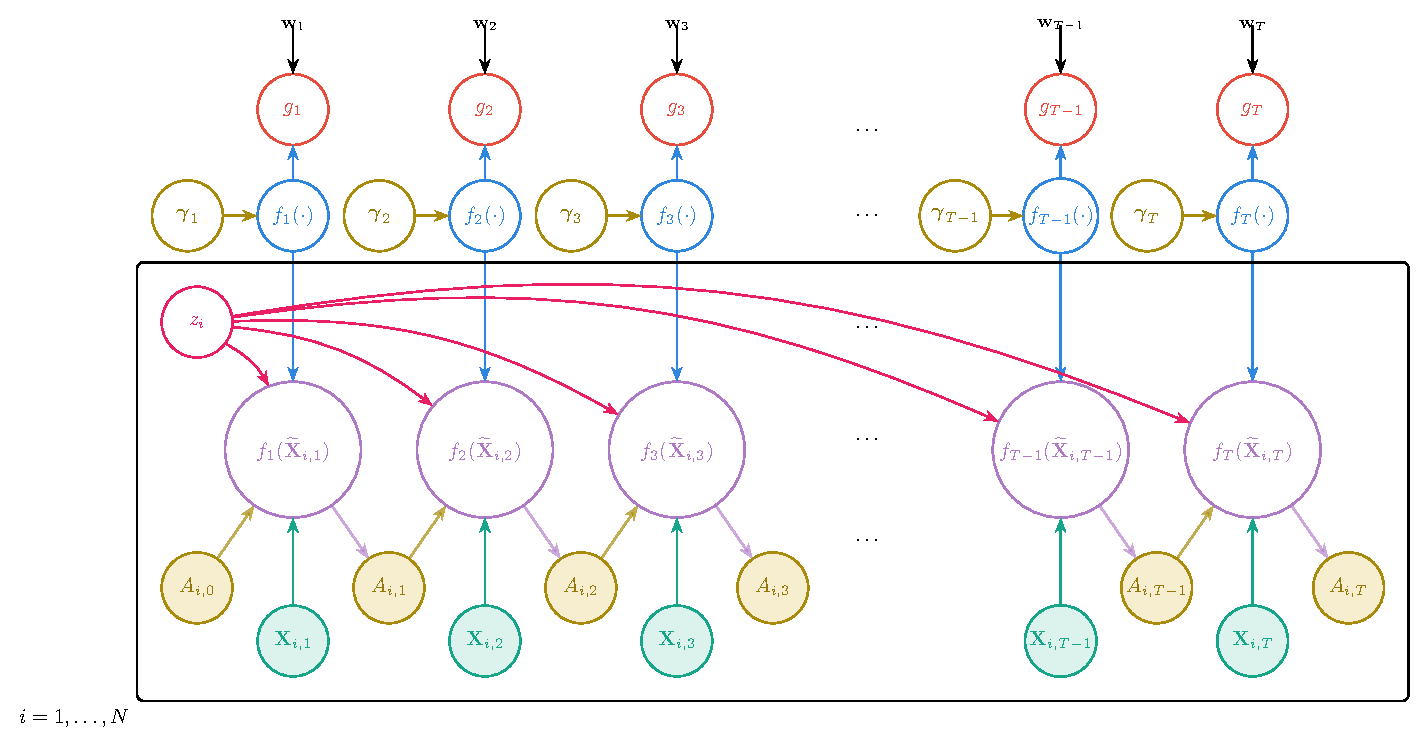
\includegraphics[width=\paperwidth,trim=0.5cm 0.5cm 0.5cm 0.5cm,
  clip]{figures/build/fit_seqgplvm_dag.pdf}
  \caption{Inference dag for the SeqGPLVM.}
  \label{fig:seqdecon-dag}
\end{figure}
\end{landscape}

\end{comment}

